\documentclass[11pt]{article}
\usepackage{amsmath,amsthm,amsfonts,amssymb,amscd}
\usepackage{cancel}
\usepackage[shortlabels]{enumitem}
\usepackage{fancyhdr} 
\usepackage{fullpage}
\usepackage[top=2cm, bottom=4.5cm, left=2.5cm, right=2.5cm]{geometry}
\usepackage{graphicx}
\usepackage{hyperref}
\usepackage{listings} %for code
\usepackage{mathtools}
\usepackage{multicol}
\usepackage{pgfplots}
\usepackage{tabularx}
\usepackage{tikz-cd,tikz}
\usepackage{todonotes}
    \pgfplotsset{
        compat=1.12,
    }
\usepackage[breakable,skins,most]{tcolorbox}
\usepackage{verbatim}
\usepackage{xcolor}
\usepackage{ytableau}

\newtcolorbox{greybox}[1]{%untitled
colback=gray!5!white,
colframe=gray!75!black,
fonttitle=\bfseries,
title=#1}

\newtcolorbox{defbox}[1]{%untitled
colback=blue!5,
colframe=blue!50,
fonttitle=\bfseries,
title=#1}

\newtcolorbox{exbox}[1]{
colback=green!5,
colframe=green!75!black,
fonttitle=\bfseries,
title=Example {(#1)}}

\newtcolorbox{pbox}[1]{
colback=violet!5,
colframe=violet!50,
fonttitle=\bfseries,
title=Proposition #1}

\newtcolorbox{quesbox}{
colback=magenta!5,
colframe=magenta!50,
fonttitle=\bfseries,
title=??}

\newtcolorbox{qbox}{
colback=red!5,
colframe=red!75,
fonttitle=\bfseries,
title=Question}

\newtcolorbox{thbox}[1]{
colback=violet!5,
colframe=violet!75,
fonttitle=\bfseries,
title=Theorem (#1)}

\hypersetup{%
  colorlinks=true,
  linkcolor=blue,
  linkbordercolor={0 0 1}
}
 
\setlength{\parindent}{0.0in}
\setlength{\parskip}{0.05in}

% Edit these as appropriate
\newcommand\course{UCI 2024}             
\newcommand\Name{Max LaFortune}

% Macros
\newcommand{\A}{\mathbb{A}}
\newcommand{\C}{\mathbb{C}}
\newcommand{\F}{\mathbb{F}}
\newcommand{\calH}{\mathcal{H}}
\newcommand{\calM}{\mathcal{M}}
\newcommand{\N}{\mathbb{N}}
\newcommand{\calP}{\mathcal{P}}
\newcommand{\Q}{\mathbb{Q}}
\newcommand{\R}{\mathbb{R}}
\newcommand{\Z}{\mathbb{Z}}

\newcommand{\all}{\ \forall \ }
\newcommand{\ans}{\textbf{A: \ }}
\newcommand{\aut}{\text{Aut}}
\newcommand{\blue}[1]{\textcolor{blue}{#1}}
\newcommand{\bs}{\backslash}
\newcommand{\cross}{\times}
\newcommand{\Def}[2]{\begin{defbox}{#1}{#2}
\end{defbox}}
\newcommand{\defn}{\textbf{\underline{Definition}}}
\newcommand{\ex}[2]{\begin{exbox}{#1}{#2}
\end{exbox}}
\newcommand{\exist}{ \ \exists \ }
\newcommand{\ext}{\text{Ext}}
\newcommand{\facts}{\textbf{\underline{Facts}}}
\newcommand{\green}[1]{\textcolor{green}{#1}}
\newcommand{\Hom}{\text{Hom}}
\newcommand{\id}[1]{\begin{quesbox}{#1}
\end{quesbox}}
\newcommand{\iso}{\cong}
\newcommand{\kw}[1]{\textit{#1}}
\newcommand{\la}{\lambda}
\newcommand{\prop}[2]{\begin{pbox}{#1}{#2}
\end{pbox}}
\newcommand{\Ques}[1]{\begin{qbox}{#1}
\end{qbox}}
\newcommand{\red}[1]{\textcolor{red}{#1}}
\newcommand{\sect}[1]{\section*{#1}}
\newcommand{\ssect}[1]{\subsection*{#1}}
\newcommand{\thm}[2]{\begin{thbox}{#1}{#2}
\end{thbox}}

\title{}
\pagestyle{fancyplain}
\headheight 35pt
\lhead{\Name}
\chead{\textbf{\Large Fixed Multiplicity}}
\rhead{\course}
\lfoot{}
\cfoot{}
\rfoot{\small\thepage}
\headsep 1.5em

\setcounter{tocdepth}{3}
\setcounter{secnumdepth}{3}

\begin{document} 
%\tableofcontents

\section*{Background}
%\addcontentsline{toc}{section}{Background}
\begin{table}[!h]
    \centering
    \begin{tabularx}{\textwidth}{c|X}
        Notation & Definition \\
        \hline \\
         $Ap(S;n)$ & $= \{ x \in S | x - n \not \in S \}$ The Apery set. \\
         $eg(S)$ & # of effective generators of $S$ \\
         $e(S)$ & embedding dimension of $S$, i.e. the number of minimal generators of $S$ \\
         $F(S)$ & Frobenius number of $S$ \\
         $g(S)$ & genus of $S$, i.e. number of gaps of $S$ \\
         $m(S)$ & multiplicity of $S$, i.e. the smallest minimal generator of $S$ \\
         $N(g)$ & \# of semigroups with genus $S$ \\
         $\langle n_1,..., n_k \rangle$ & numerical semigroup generated by $\{n_1, ...,n_k\}$
    \end{tabularx}
\end{table}

Each numerical semigroup corresponds to a unique Kunz Coordinate. Consider some numerical semigroup $S$ with $m(S) = m$. Then $S$ has the Apery set $Ap(S) = \{m, mk_1 + 1, mk_2 + 2, \dots, mk_{m-1} + (m-1) \}$ and the associated Kunz coordinates $(k_1, k_2, \dots, k_{m-1}).$ Semigroups of multiplicity $m$ are integer points in the Kunz Polyhedra $P_m \subseteq \R ^{m-1}$.  

The bounding inequalities for the Kunz polyhdrom $P_m \subseteq \R^{m-1}$ are 
$$x_i + x_j \geq x_{i+j} \ \text{for} \ 1 \leq i \leq j \leq m - 1 \ \text{with} \ i + j < m$$
$$x_i + x_j + 1 \geq x_{i+j-m} \ \text{for} \ 1 \leq i \leq j \leq m - 1 \ \text{with} \ i + j > m$$

\underline{\textbf{Theorem (O'Dorney)}}
$$\lim_{g \to \infty} \frac{\# \{S | g(S) = g, eg(S) = h \}}{N(g)} = \frac{1}{\varphi^{n+2}}$$

\underline{\textbf{Question}} \\
What would happen if you look at semigroups of fixed multiplicity? \\
So for a fixed $m$ what is $$\lim_{g \to \infty} \frac{\# \{S | g(S) = g, m(S)=m, eg(S) = h \}}{\# \{ S | g(S) = g, m(S) = m\}} ?$$



\section*{Multiplicity 3}
%\addcontentsline{toc}{section}{Multiplicity 3}
If $S \to (k_1, k_2)$ then the children of $S$ will be 
\begin{itemize}
    \item $(k_1 + 1, k_2)$ when $k_2 + 1 \leq k_1 < 2k_2 + 1$,
    \item $(k_1, k_2 + 1)$ when $k_1 \leq k_2 < 2k_1$.
\end{itemize}
Note: If $k_1=k_2$ or $k_1 = k_2 + 1$ both $(k_1 + 1, k_2)$ and $(k_1, k_2 + 1)$ will be children. If $k_1 = 2k+1$ or $k_2 = 2k_1$ there will be no children.

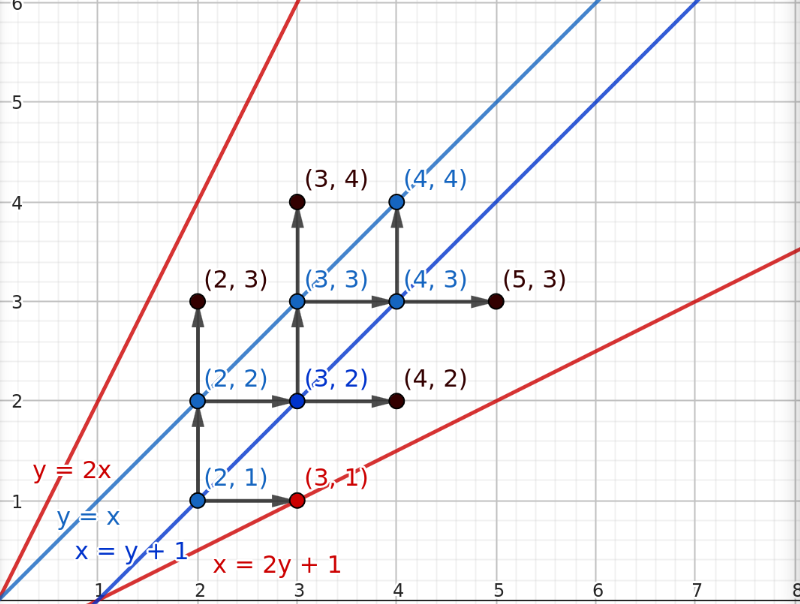
\includegraphics[scale=0.3]{Max/images/Screenshot from 2024-07-15 13-01-52.png}

We can show that for semigroups of multiplicity 3 and $h > 0$ we have 
$$\lim_{g \to \infty} \frac{\# \{S | g(S) = g, eg(S) = h \}}{\# \{ S | g(S) = g\}} = 1$$


%\section*{Multiplicity 4}
%\addcontentsline{toc}{section}{Multiplicity 4}

\input{Max/FixedMult/M4}










\end{document}